\documentclass[11pt]{article}
\usepackage[a4paper,margin=0.88in]{geometry}
\usepackage{amsmath,amssymb,amsthm}
\usepackage{graphicx}
\usepackage{float}
\usepackage{microtype}
\usepackage[hidelinks]{hyperref}
\emergencystretch=3em

\newcommand{\Dmu}{\mathcal D_\mu}
\newcommand{\T}{\mathbb T}
\newcommand{\D}{\mathbb D}

\title{The support--spectrum disjointness condition is not necessary\\[0.3em]
\large A literature-implied negative answer to arXiv:2310.03604}
\author{Automated Mathematics Run \texttt{fa\_banach\_001}, lane 0}
\date{11 August 2026}

\begin{document}
\maketitle

\begin{center}
\fbox{\parbox{0.92\linewidth}{\textbf{Status: literature already implies a
negative answer.} No new theorem is claimed.  The explicit example in
arXiv:2509.04907 has a bounded embedding
$K_u\hookrightarrow\mathcal D_\mu$ while
$\operatorname{supp}\mu\cap\sigma(u)=\{1\}\ne\varnothing$.}}
\end{center}

\section{The source problem}

For an inner function $u$, write
$K_u=H^2\ominus uH^2$ and let $\sigma(u)$ be its boundary spectrum.  For a
finite positive Borel measure $\mu$ on $\T$, the harmonically weighted
Dirichlet seminorm disintegrates as
\[
 D_\mu(f)=\int_{\T}D_\zeta(f)\,d\mu(\zeta).
\]
Bellavita--Dellepiane prove that
\[
 \operatorname{supp}\mu\cap\sigma(u)=\varnothing
 \quad\Longrightarrow\quad K_u\hookrightarrow\Dmu,
\]
and that the embedding forces $\mu(\sigma(u))=0$.  They ask whether the
stronger support-disjointness condition is necessary in general.

\begin{figure}[H]
  \centering
  
\includegraphics[width=0.88\linewidth]{figures/source_open_problem.png}
  \caption{The exact open problem on source PDF page 15 of
  arXiv:2310.03604v3.}
\end{figure}

\section{The later explicit example}

Bellavita--Dellepiane--Hartmann--Mashreghi, arXiv:2509.04907, take the
singular inner function
\[
 u(z)=\exp\!\left(\frac{z+1}{z-1}\right),
 \qquad \sigma(u)=\rho(u)=\{1\}.
\]
Its Clark atoms are
\[
 \zeta_n=\frac{2\pi i n+1}{2\pi i n-1},\qquad n\in\mathbb Z,
\]
and they define
\[
 \mu=\sum_{n\in\mathbb Z}\frac{1}{|u'(\zeta_n)|^2}\,\delta_{\zeta_n}.
\]
The paper verifies the required potential estimate and, in Theorem~8.3,
proves
\[
 \mathcal H\!\left(\frac{1+u}{2}\right)=\Dmu.
\]

\begin{figure}[H]
  \centering
  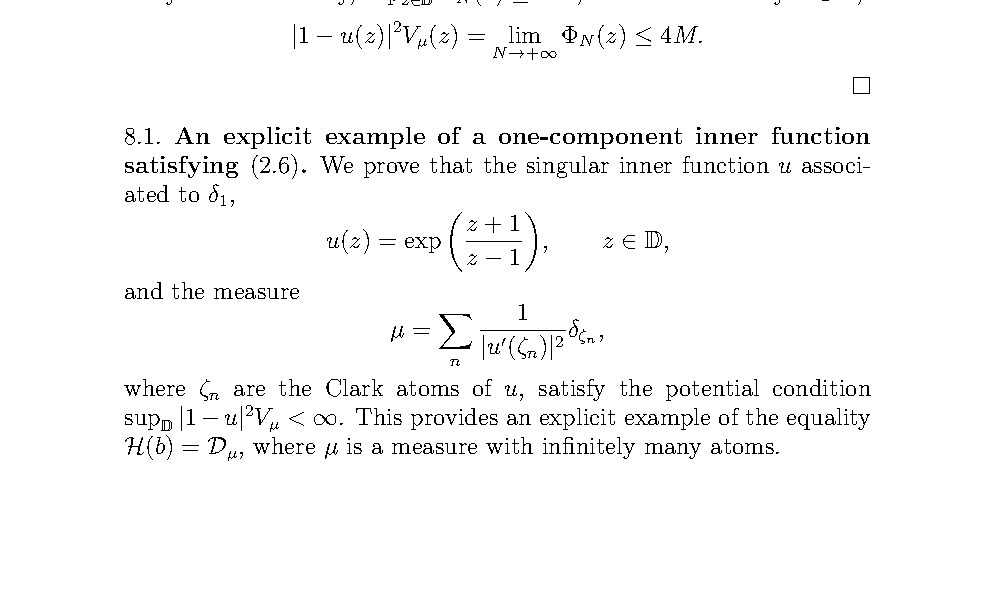
\includegraphics[width=0.78\linewidth]{figures/answer_construction.png}
  \caption{The construction on supporting PDF page 35 of
  arXiv:2509.04907v1.}
\end{figure}

The implication needed here is explicit in that paper.  In the proof of its
Theorem~6.3, after treating the $aH^2$ component, the authors separately prove
$K_u\hookrightarrow\Dmu$.

\begin{figure}[H]
  \centering
  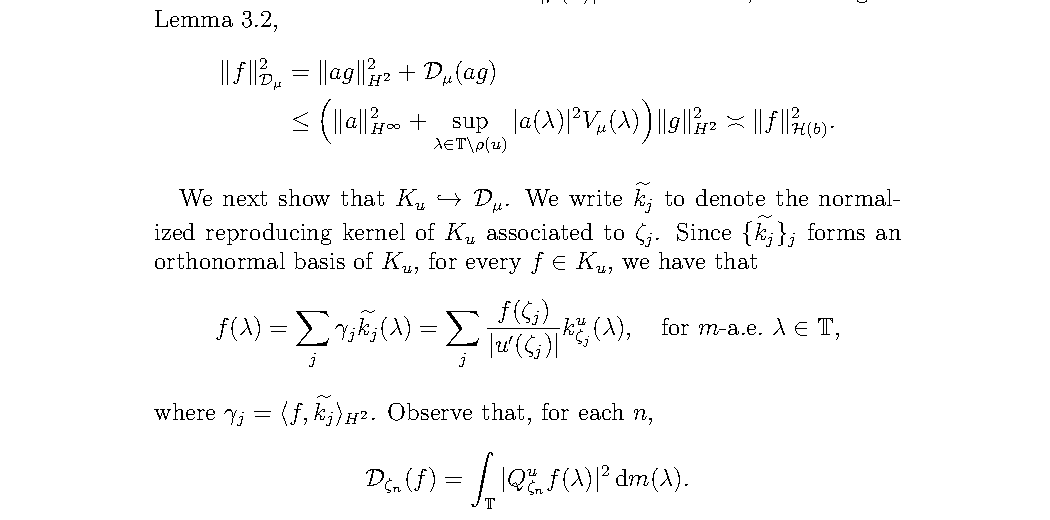
\includegraphics[width=0.84\linewidth]{figures/answer_embedding_step.png}
  \caption{The component-embedding step on supporting PDF page 27.}
\end{figure}

\section{Why this negates the source condition}

Every coefficient of $\mu$ is positive.  Moreover,
\[
 \zeta_n-1=\frac{2}{2\pi i n-1}\longrightarrow0
 \quad (|n|\to\infty),
\]
so every neighbourhood of $1$ has positive $\mu$-mass.  Hence
$1\in\operatorname{supp}\mu$.  No atom is placed at $1$, and the paper
computes
\[
 \frac1{|u'(\zeta_n)|}
 =\frac{2}{4\pi^2n^2+1},
\]
so $\mu$ is finite and $\mu(\{1\})=0$.  Therefore
\[
 K_u\hookrightarrow\Dmu,
 \qquad
 \mu(\sigma(u))=0,
 \qquad
 \operatorname{supp}\mu\cap\sigma(u)=\{1\}.
\]
This is exactly a counterexample to necessity of the source's sufficient
condition, while sharply respecting its proved necessary condition.

\section{Crosswalk and conclusion}

The notation $\rho(u)$ in arXiv:2509.04907 is the same closed boundary
spectrum that arXiv:2310.03604 denotes by $\sigma(u)$: for inner $u$ it is
the set of boundary points where $\liminf_{z\to\zeta}|u(z)|=0$.  Thus there
is no hypothesis mismatch.  The later article does not advertise its example
as an answer to the 2023 final question, so this packet classifies the answer
as \texttt{literature\_implied}, not as a new counterexample.

\begin{thebibliography}{9}
\bibitem{BD2025}
C.~Bellavita and E.~Dellepiane,
\emph{Embedding model and de Branges--Rovnyak spaces in Dirichlet spaces},
Complex Variables and Elliptic Equations 70 (2025), 228--246;
arXiv:2310.03604.

\bibitem{BDHM2025}
C.~Bellavita, E.~Dellepiane, A.~Hartmann, and J.~Mashreghi,
\emph{Infinitely supported harmonically weighted Dirichlet spaces which are
de Branges--Rovnyak spaces}, arXiv:2509.04907 (2025).
\end{thebibliography}

\end{document}
